\documentclass[10pt,a4paper]{article}
\renewcommand{\baselinestretch}{1.0}
\usepackage{cite}
\usepackage[dvips]{graphicx}
\usepackage{psfrag}
\usepackage{color}
\usepackage[cmex10]{amsmath}
\usepackage{amsfonts}
\usepackage[font=footnotesize, captionskip=10pt]{subfig}
\usepackage{tikz}
\usepackage{flushend}
\usepackage{times}
\usepackage[margin=1.5cm]{geometry}
\usepackage[slovak]{babel}
\usepackage[utf8]{inputenc}
\usepackage[T1]{fontenc}
\usepackage[]{algorithm2e}


\pagestyle{empty}

\hyphenation{net-works}
\newtheorem{remark}{Remark}

\begin{document}

\title{Popis experimentov}
\author{autor a,b,c,d}
\date{}
\maketitle
\thispagestyle{empty}


\section{Popis experimentov}

Pre tréning všetkých variánt exeprimentov boli zvolené rovnaké hyperparametre,
rýchlosť učenia $\eta = 0.1$, strmosť báz $k = 0.02$.
Počet epoch učenia bol zvolený na $50$, čo poskytuje istotu že váhy siete budú dotrénované
(s ohľadom na veľkosť $\eta$ a počet dát).

Pre počty báz sme experimentovali s počtami $256$, $1024$, $4096$ a $8192$.

Celkovo boli k dispozícií dáta z 5 experimentov (4 rôznych kanálov).

\begin{table}[!ht]
\begin{tabular}{|l|l|}
\hline
ID & popis                     \\ \hline
0  & kanal\_kika\_sim6         \\ \hline
1  & kanal\_kika\_sim6\_modulo \\ \hline
2  & kanal\_kika\_sim101       \\ \hline
3  & kanal\_mato\_sim50        \\ \hline
4  & kanal\_monika\_sim3044    \\ \hline
\end{tabular}
\end{table}

Kanály 0 a 1 sú ten istý kanál, v časti modulo sme využili periodicitu kanála
a umelo sme tak zväčšili množstvo trénovacích dát približne 3 krát.
Kanál 2 je varainta predošlých dvoch, ale bola odstránená jedna prekážka.
O kanáloch 3 a 4 neviem čo by som povedal.

Pre každý experiment sa zvolila tránovacia a testovacia množina - na tento účel
poslúžil rôzny seed z daného kanála.
Všetky experimenty boli trénované na seede A a testované na seede B.
Pre počet báz 4096 boli navyše zvolené varianty trénovacej a testovacej množiny podľa nasledujúcej tabuľky

\begin{table}[!ht]
\begin{tabular}{|l|l|l|l|}
\hline
Varianta & Popis             & Training seed & Testing seed \\ \hline
0        & regular           & A             & B            \\ \hline
1        & swap              & B             & A            \\ \hline
2        & verification      & A             & A            \\ \hline
3        & verification swap & B             & B            \\ \hline
\end{tabular}
\end{table}

Pre predikciu trajektórií má najväčší význam varianta 0 (klasická regresná úloha pre ML), ostatné slúžia pre štatistickú
verifkáciu modelu.


\section{Výsledky pre ID 0}

Prepovedané trajektórie a ich chyby pre rôzne počty báz

\begin{figure}[!ht]
\centering
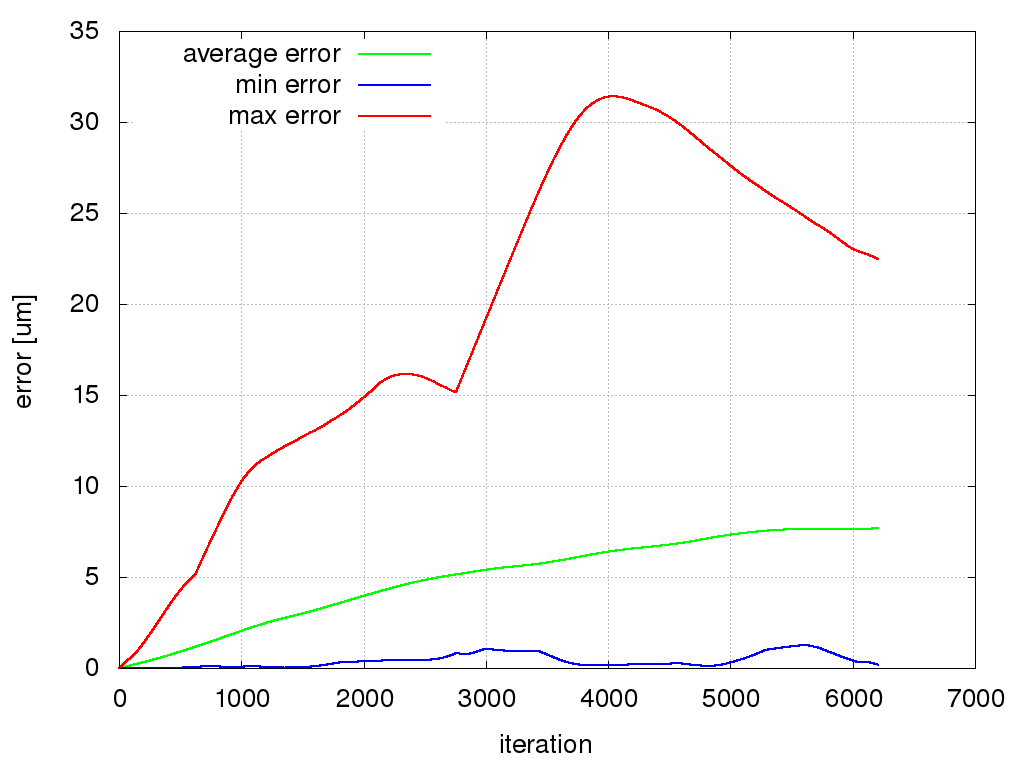
\includegraphics[width=8cm]{images/kanal_kika_sim6/256_basis/summary_error_during_trajectory_reconstruction.png}
\caption{Chyba predpovede pre 256 báz}
\label{img:id_0_prediction_error_256_basis}
\end{figure}

\begin{figure}[!ht]
\centering
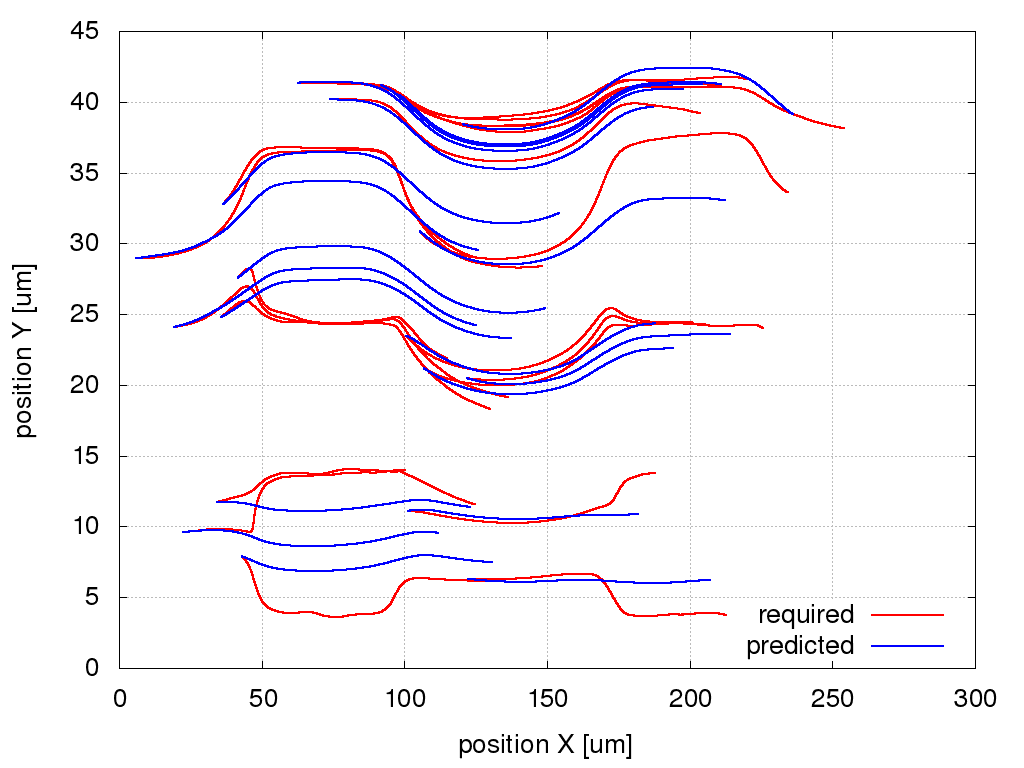
\includegraphics[width=8cm]{images/kanal_kika_sim6/256_basis/trajectory_prediction_for_20_cells.png}
\caption{Predikcia dráhy pre prvých 20 buniek a 256 báz}
\label{img:id_0_prediction_256_basis}
\end{figure}

\begin{figure}[!ht]
\centering
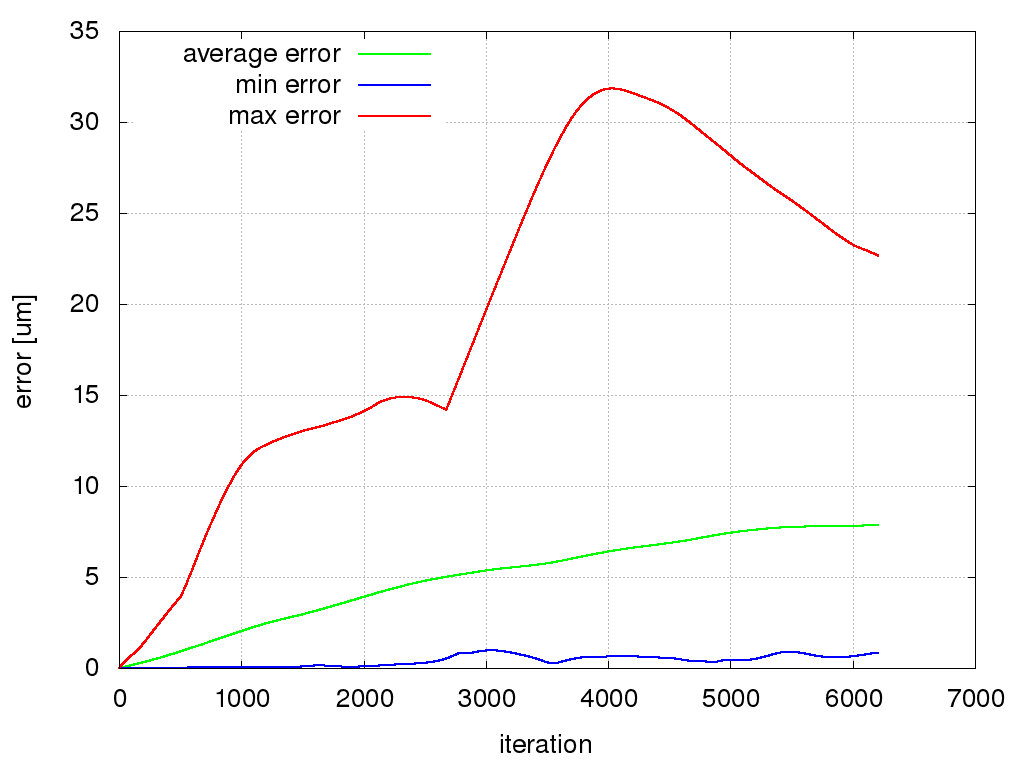
\includegraphics[width=8cm]{images/kanal_kika_sim6/1024_basis/summary_error_during_trajectory_reconstruction.png}
\caption{Chyba predpovede pre 1024 báz}
\label{img:id_0_prediction_error_1024_basis}
\end{figure}

\begin{figure}[!ht]
\centering
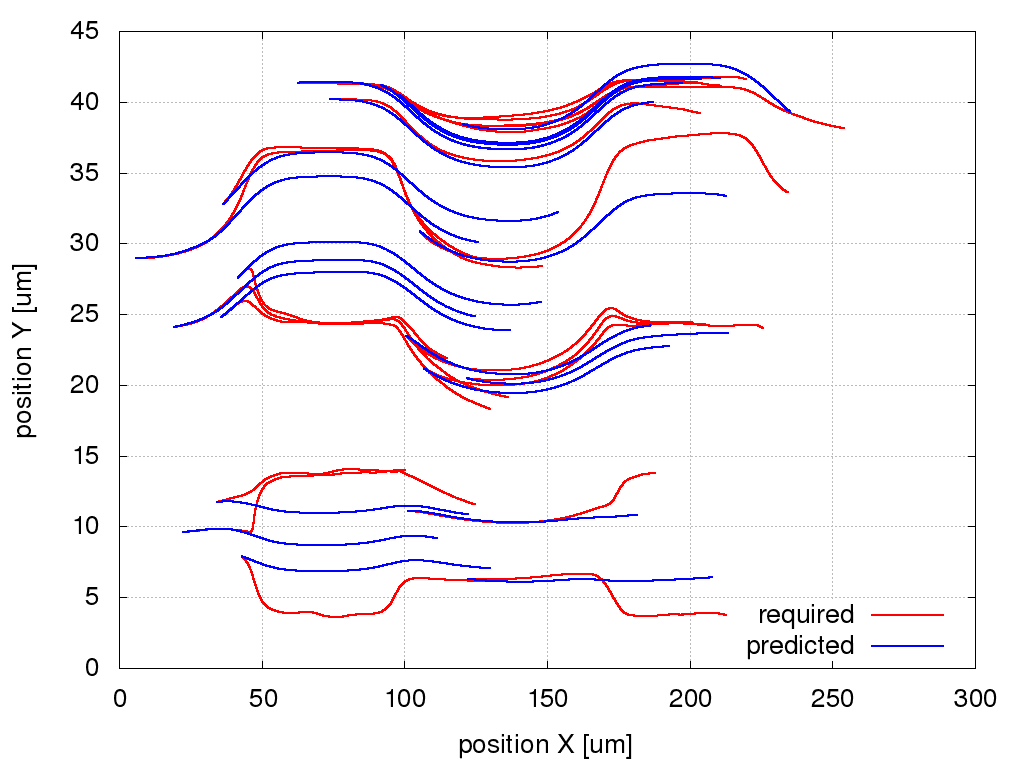
\includegraphics[width=8cm]{images/kanal_kika_sim6/1024_basis/trajectory_prediction_for_20_cells.png}
\caption{Predikcia dráhy pre prvých 20 buniek a 1024 báz}
\label{img:id_0_prediction_1024_basis}
\end{figure}

\begin{figure}[!ht]
\centering
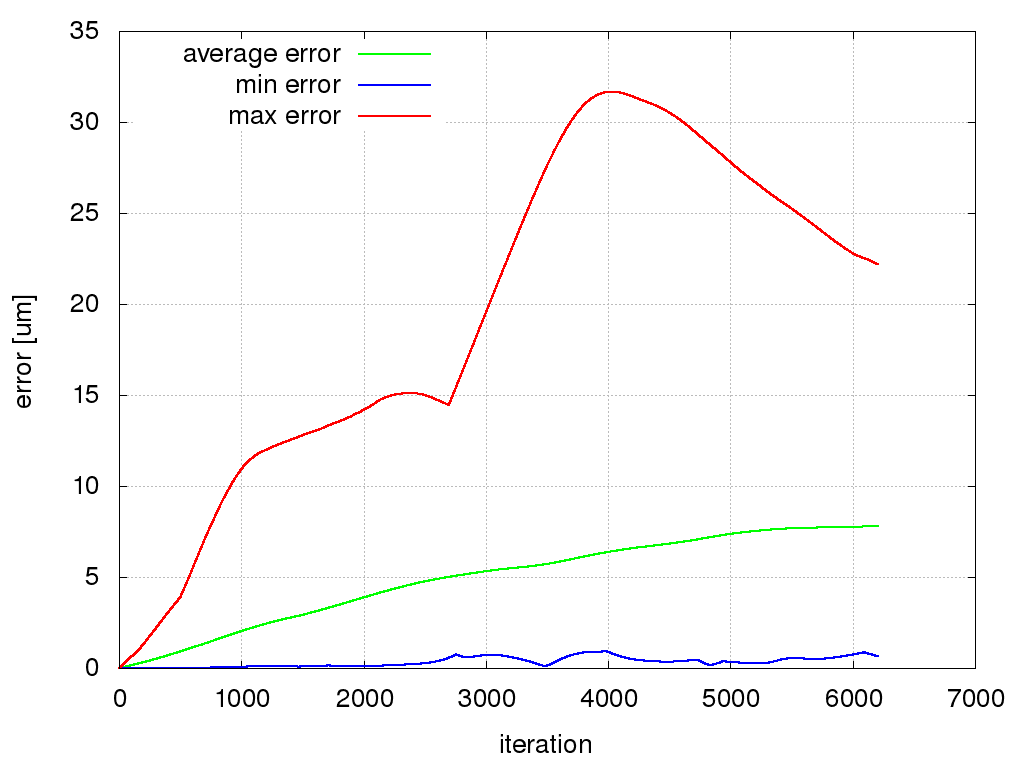
\includegraphics[width=8cm]{images/kanal_kika_sim6/4096_basis/summary_error_during_trajectory_reconstruction.png}
\caption{Chyba predpovede pre 4096 báz}
\label{img:id_0_prediction_error_4096_basis}
\end{figure}

\begin{figure}[!ht]
\centering
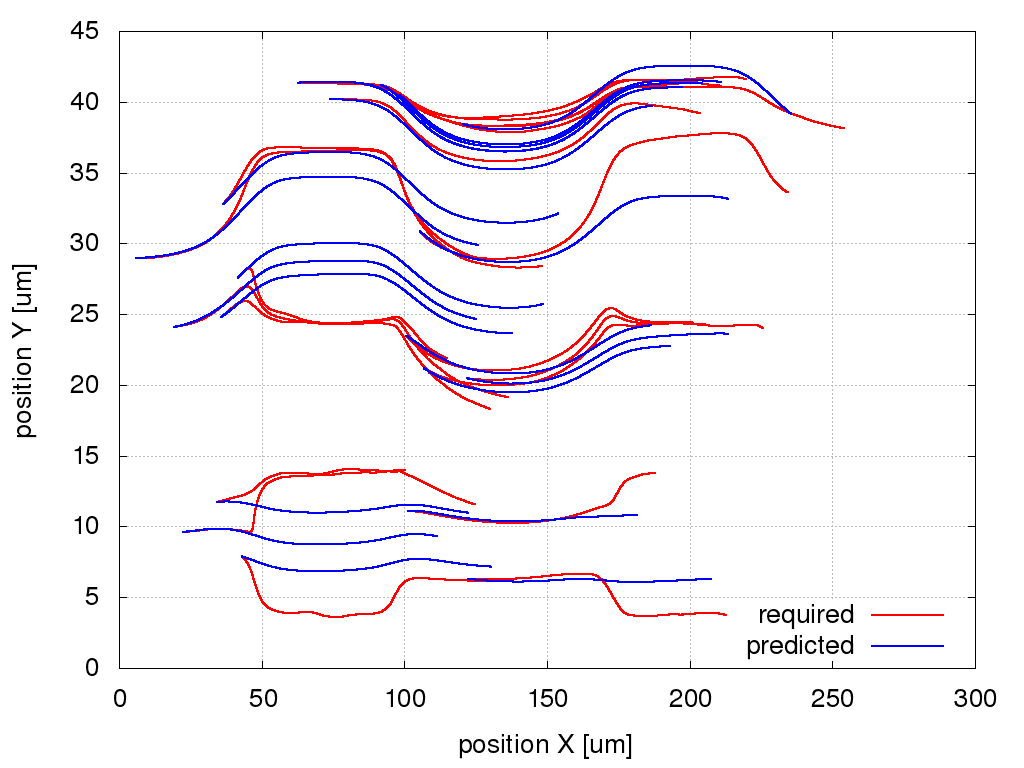
\includegraphics[width=8cm]{images/kanal_kika_sim6/4096_basis/trajectory_prediction_for_20_cells.png}
\caption{Predikcia dráhy pre prvých 20 buniek a 4096 báz}
\label{img:id_0_prediction_4096_basis}
\end{figure}

\begin{figure}[!ht]
\centering
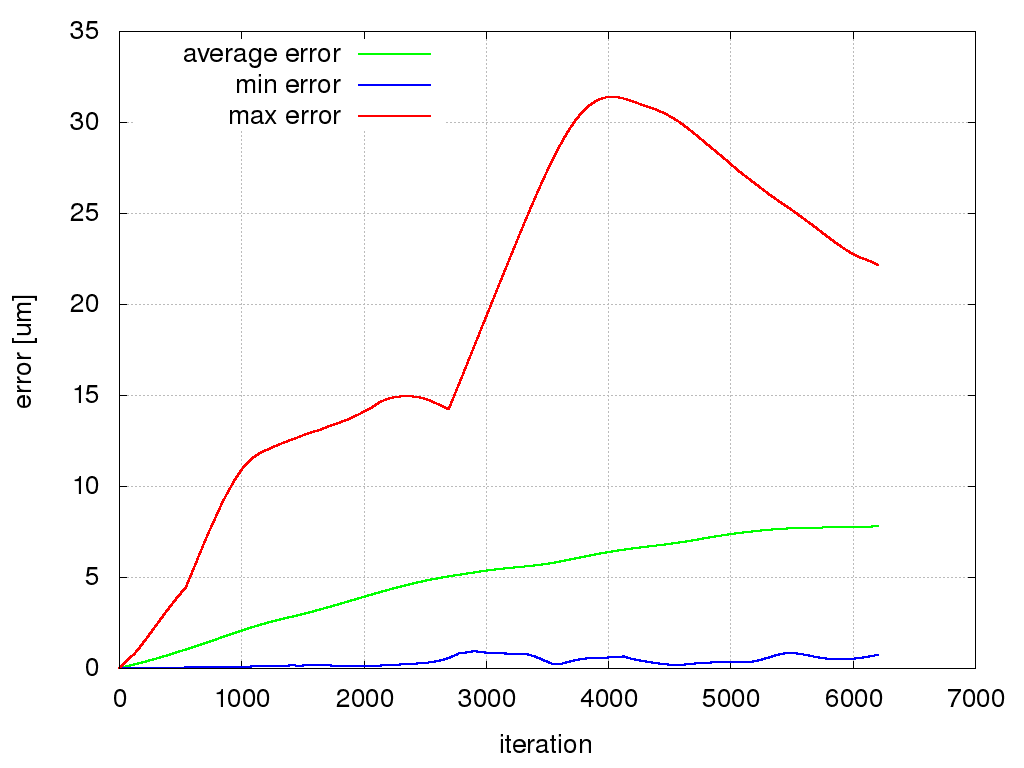
\includegraphics[width=8cm]{images/kanal_kika_sim6/8192_basis/summary_error_during_trajectory_reconstruction.png}
\caption{Chyba predpovede pre 8192 báz}
\label{img:id_0_prediction_error_8192_basis}
\end{figure}

\begin{figure}[!ht]
\centering
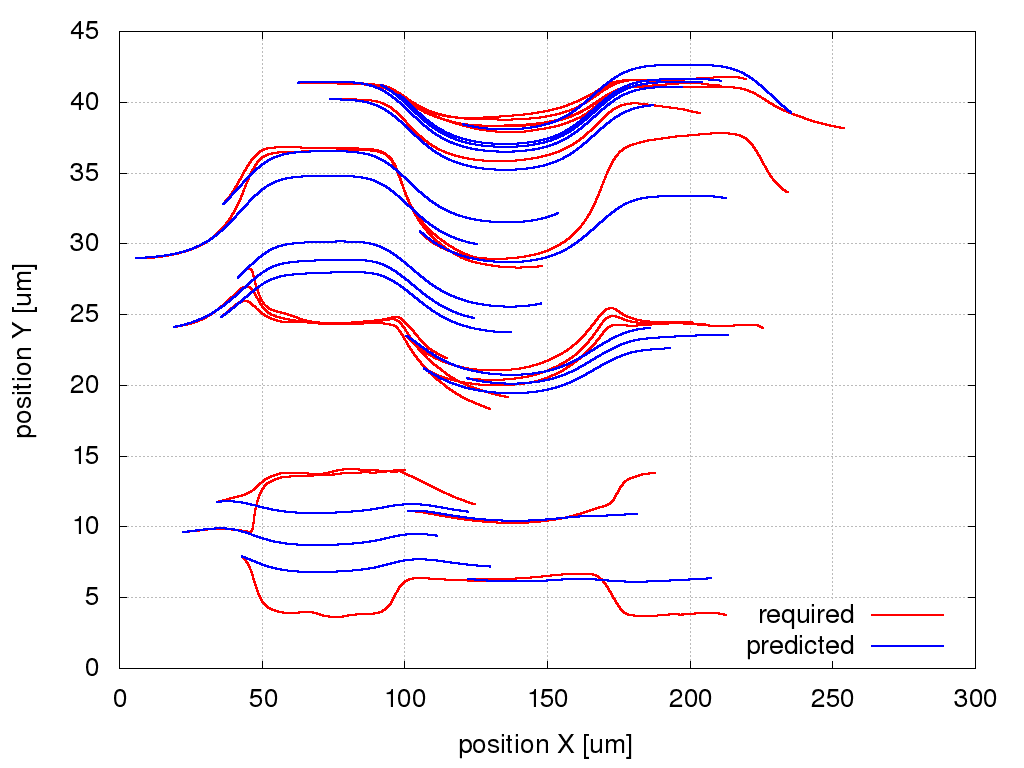
\includegraphics[width=8cm]{images/kanal_kika_sim6/8192_basis/trajectory_prediction_for_20_cells.png}
\caption{Predikcia dráhy pre prvých 20 buniek a 8192 báz}
\label{img:id_0_prediction_8192_basis}
\end{figure}

%\begin{figure}[!ht]
%\centering
%\includegraphics[width=8cm]{images/e6_approximation_size.png}
%\caption{experiment 6}
%\label{img:experiment6}
%\end{figure}














\begin{thebibliography}{9}
\bibitem{bib:kohonen_network}
R. Rojas: Neural Networks, Springer-Verlag, Berlin, 1996, Kohonen Networks

\bibitem{bib:gradient_descent}
Sebastian Ruder, An overview of gradient descent optimization algorithms
\end{thebibliography}




\end{document}
